\section{Использование коллекций (Задание 7 вариант 8)}

\subsection{Условие задания}

Создать очередь, состоящую из целых чисел. Предусмотреть возможность создания очереди из набора чисел, добавления одного элемента (функция push), удаления одного элемента (функция pop), вывода результата на экран, удаления всех элементов с помощью кнопок. Найти сумму четных элементов, попадающих в заданный интервал [a, b]. Получить новую очередь, вставив после максимальных элементов новый элемент.

Приложение должно содержать следующие пункты:

\begin{enumerate}
    \item{Заголовок формы должен отражать суть задания.}
    \item{Все элементы формы должны быть внятно подписаны (кнопки подписаны, у тестового поля должно быть написано, для чего оно нужно и т. д.)}
    \item{В коде должны быть комментарии и отступы (код должен быть легко читаем).}
    \item{В коде программы все элементы формы должны быть переименованы (btnName ---  для кнопок, lblName --- для ссылок, txtName --- для текстового поля и т. д.) Наименования должны быть понятными.}
    \item{Должна быть возможность для ввода и вывода первоначальных данных.}
    \item{Должна быть возможность для вставки и удаления одного элемента.}
    \item{Должны использоваться коллекции.}
    \item{Ответы на задания должны быть в разных полях.}
    \item{Если нет данных для выполнения задания, выводить соответствующие данные.}
    \item{Для графов использовать список смежности.}
\end{enumerate}

\subsection{Вид формы в конструкторе}

Форма имеет вид (рис.\ref{fig:FormInConstruct7}):

\newpage

\begin{figure}[!h]
    \centering
    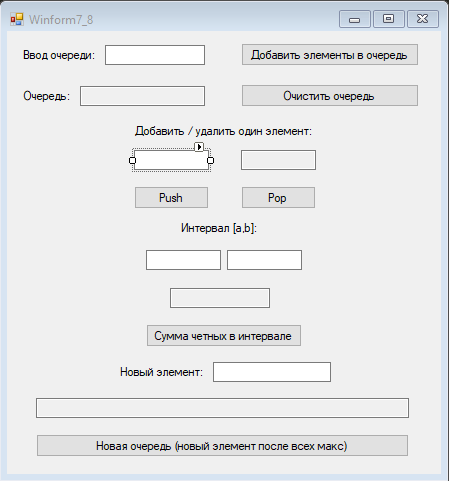
\includegraphics[width = 0.5\textwidth]{images/Task7/FormInConstructor.png}
    \caption{Вид формы в конструкторе}
    \label{fig:FormInConstruct7}
\end{figure}

\subsection{Таблица с описанием переименовнных элементов формы}

Все элементы формы были переименованы и их атрибыты изменены. Проведенные изменения представлены в таблице \ref{tab:label7}

\begin{longtable}[!h]{|l|l|l|}
    \caption{Значения атрибутов элементов в приложении <<Использование коллекций>>}
    \label{tab:label7}
    \endfirsthead
    \endhead
    \hline
    \makecell{$\textbf{Описание элементов}$\\ $\textbf{формы}$}& \makecell{$\textbf{Список измененных}$\\ $\textbf{атрибутов}$}& \makecell{$\textbf{Новое значение}$\\ $\textbf{атрибута}$}\\ 
    \hline
    \makecell{Форма}& \makecell{Text}& \makecell{Использование\\ коллекций}\\ 
    \hline
    \makecell{Первая надпись (label)}& \makecell{Name}& \makecell{lbl1}\\ 
    \hline
    \makecell{Первая надпись (label)}& \makecell{Text}& \makecell{Ввод очереди:}\\ 
    \hline
    \makecell{Вторая надпись (label)}& \makecell{Name}& \makecell{lbl2}\\ 
    \hline
    \makecell{Вторая надпись (label)}& \makecell{Text}& \makecell{Очередь:}\\ 
    \hline
    \makecell{Третья надпись (label)}& \makecell{Name}& \makecell{lbl3}\\ 
    \hline
    \makecell{Третья надпись (label)}& \makecell{Text}& \makecell{Добавить/удалить\\ один элемент:}\\ 
    \hline
    \makecell{Четвёртая надпись (label)}& \makecell{Name}& \makecell{lbl4}\\ 
    \hline
    \makecell{Четвёртая надпись (label)}& \makecell{Text}& \makecell{Интервал [a, b]}\\ 
    \hline
    \makecell{Пятая надпись (label)}& \makecell{Name}& \makecell{lbl5}\\ 
    \hline
    \makecell{Пятая надпись (label)}& \makecell{Text}& \makecell{Новый элемент:}\\ 
    \hline
    
    \makecell{Первое текстовое\\ поле (textBox)}& \makecell{Name}& \makecell{tBInputQue}\\ 
    \hline
    \makecell{Второе текстовое\\ поле (textBox)}& \makecell{Name}& \makecell{tBOutputQue}\\ 
    \hline
    \makecell{Второе текстовое\\ поле (textBox)}& \makecell{ReadOnly}& \makecell{True}\\ 
    \hline
    \makecell{Третье текстовое\\ поле (textBox)}& \makecell{Name}& \makecell{tBInputPush}\\ 
    \hline
    \makecell{Четвёртое текстовое\\ поле (textBox)}& \makecell{Name}& \makecell{tBOutputPop}\\ 
    \hline
    \makecell{Четвёртое текстовое\\ поле (textBox)}& \makecell{ReadOnly}& \makecell{True}\\ 
    \hline
    \makecell{Пятое текстовое\\ поле (textBox)}& \makecell{Name}& \makecell{tBInputA}\\ 
    \hline
    \makecell{Шестое текстовое\\ поле (textBox)}& \makecell{Name}& \makecell{tBInputB}\\ 
    \hline
    \makecell{Седьмое текстовое\\ поле (textBox)}& \makecell{Name}& \makecell{tBOutputSum}\\ 
    \hline
    \makecell{Седьмое текстовое\\ поле (textBox)}& \makecell{ReadOnly}& \makecell{True}\\ 
    \hline
    \makecell{Восьмое текстовое\\ поле (textBox)}& \makecell{Name}& \makecell{tBInputNAM}\\ 
    \hline
    \makecell{Девятое текстовое\\ поле (textBox)}& \makecell{Name}& \makecell{tBOutputNAM}\\ 
    \hline
    \makecell{Девятое текстовое\\ поле (textBox)}& \makecell{ReadOnly}& \makecell{True}\\ 
    \hline

    \makecell{Первая кнопка (button)}& \makecell{Name}& \makecell{btnInputQue}\\ 
    \hline
    \makecell{Первая кнопка (button)}& \makecell{Text}& \makecell{Добавить элементы\\ в очередь}\\ 
    \hline
    \makecell{Вторая кнопка (button)}& \makecell{Name}& \makecell{btnClearQue}\\ 
    \hline
    \makecell{Вторая кнопка (button)}& \makecell{Text}& \makecell{Очистить очередь}\\ 
    \hline
    \makecell{Третья кнопка (button)}& \makecell{Name}& \makecell{btnPush}\\ 
    \hline
    \makecell{Третья кнопка (button)}& \makecell{Text}& \makecell{Push}\\ 
    \hline
    \makecell{Четвёртая кнопка (button)}& \makecell{Name}& \makecell{btnPop}\\ 
    \hline
    \makecell{Четвёртая кнопка (button)}& \makecell{Text}& \makecell{Pop}\\ 
    \hline
    \makecell{Пятая кнопка (button)}& \makecell{Name}& \makecell{btnSum}\\ 
    \hline
    \makecell{Пятая кнопка (button)}& \makecell{Text}& \makecell{Сумма четных\\ в интервале}\\ 
    \hline
    \makecell{Шестая кнопка (button)}& \makecell{Name}& \makecell{btnNewAfterMax}\\ 
    \hline
    \makecell{Шестая кнопка (button)}& \makecell{Text}& \makecell{Новая очередь\\ (новый элемент\\ после всех макс)}\\ 
    \hline

    \makecell{Обработчик ошибок\\ (errorProvider)}& \makecell{Name}& \makecell{eP1}\\ 
    \hline
\end{longtable}

\subsection{Примеры работы}

При запуске приложения на экране появляется окно (рис.\ref{fig:StartForm7}).

\begin{figure}[!h]
    \centering
    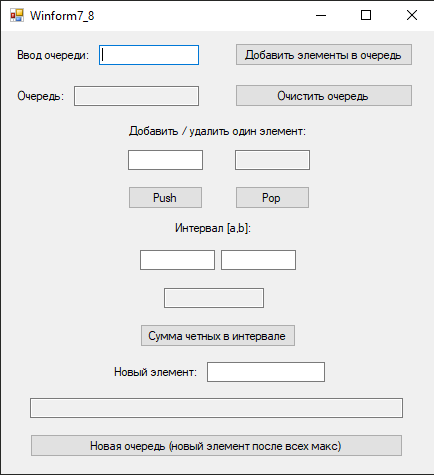
\includegraphics[width = 0.5\textwidth]{images/Task7/Start.png}
    \caption{Запуск приложения}
    \label{fig:StartForm7}
\end{figure}

При запуске с корректными данными, при нажатии на кнопку <<Добавить элементы в очередь>> происходит (рис.\ref{fig:WorkForm7}):

\newpage

\begin{figure}[!h]
    \centering
    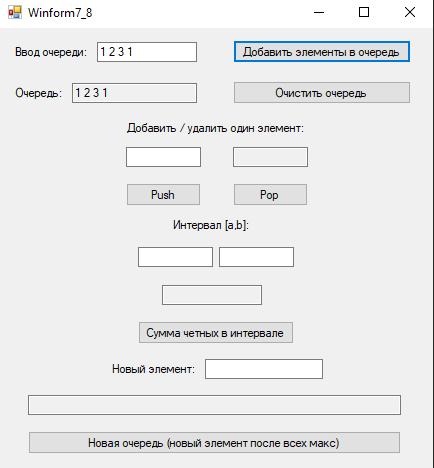
\includegraphics[width = 0.5\textwidth]{images/Task7/WorkAddQueue.png}
    \caption{Запуск с корректными данными}
    \label{fig:WorkForm7}
\end{figure}

При запуске с некорректными данными, при нажатии на кнопку <<Добавить элементы в очередь>> происходит  (рис.\ref{fig:BadInputNotIntForm7}):

\begin{figure}[!h]
    \centering
    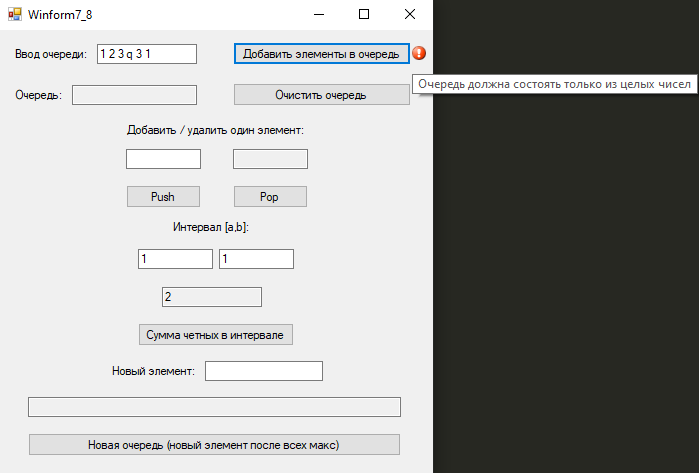
\includegraphics[width = 0.7\textwidth]{images/Task7/BadInputAddNotInt.png}
    \caption{Запуск с некорректными данными}
    \label{fig:BadInputNotIntForm7}
\end{figure}

\subsection{Примеры кода}

Функция добавления одного элемента в очередь:

\begin{minted}{c++}
		private: System::Void btnPush_Click(System::Object^ sender, System::EventArgs^ e) {
			ClearEP();
			// Вспомогательная очередь
			System::Collections::Generic::Queue<int> buffer;
			// Считываем число
			int number;
			bool res = Int32::TryParse(tBInputPush->Text, number);
			String^ str = "";
			// Проверка на число
			if (!res) {
				this->eP1->SetError(btnPush, "Не целое число");
				buffer.Clear();
				return;
			}
			q.Enqueue(number);
			QueueOutput();
		}
\end{minted}

Другие фрагменты кода расположены в приложении \ref{app:task7}. Полный код программы приведен в приложении \ref{app:zip}
